% -*- coding: utf-8 -*-
%%%%%%%%%%%%%%%%%%%%%%%%%%%%%%%%%%%%%%%%%%%%%%%%
%%%%%%%%%%%%%%%%%%%%%%%%%%%%%%%%%%%%%%%%%%%%%%%%
%%%%%%%%%%%%%%%%%%%%%%%%%%%%%%%%%%%%%%%%%%%%%%%%
\chapter{ヒューリスティック探索 (Heuristic Search)}
\label{ch:heuristic-search}

\ref{ch:blind-search}章では問題の知識を利用しないグラフ探索手法について解説した。
本章では問題の知識を利用することでより効率的なグラフ探索を行う手法、特にヒューリスティック探索について解説する。

\section{ヒューリスティックとは?}
\label{sec:heursitic}

\begin{figure}
  \centering
  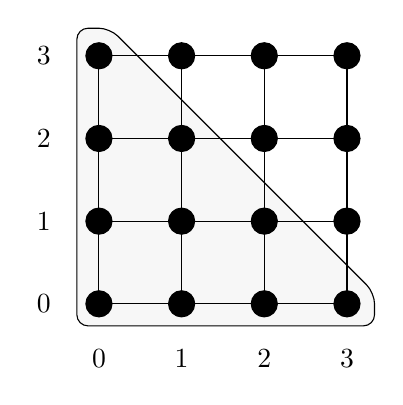
\begin{tikzpicture}[scale=0.7]
    % BrFS region

\draw[rounded corners, fill=gray!20, fill opacity=0.3] (-0.4, -0.4) -- (3*1.5+0.5, -0.4) -- (3*1.5+0.5, 0.2) -- (0.2, 3*1.5+0.5) -- (-0.4, 3*1.5+0.5) -- cycle;


% Grid pathfinding

\foreach \x in {0,...,3}
  \foreach \y in {0,...,3}
    {\node [draw, circle, fill=black] (\x\y) at (1.5*\x, 1.5*\y) {};}

\foreach \x in {0,...,3}
  \foreach \y in {0,...,2}
           {\draw (1.5 * \x, 1.5 * \y) -- (1.5 * \x, 1.5 * \y + 1.5);}

\foreach \y in {0,...,3}
  \foreach \x in {0,...,2}
           {\draw (1.5 * \x, 1.5 * \y) -- (1.5 * \x + 1.5, 1.5 * \y);}
           
\foreach \x in {0,...,3}
         {\node at (1.5 * \x, -1) {\x};
          \node at (-1, 1.5 * \x) {\x};
         }

  \end{tikzpicture}
  \caption{グリッド経路探索におけるダイクストラ法}
\label{fig:grid-brfs}  
\end{figure}

経路探索問題をダイクストラ法で解くことを考えよう。
図\ref{fig:grid-brfs}のグリッド経路探索問題で(0, 0)の位置から(3, 0)の位置まで移動するため経路を求める問題を考えよう。
このときダイクストラ法が探索していく範囲は図\ref{fig:grid-brfs}の灰色のエリアにあるノードになる。
しかし人間が経路探索を行うときにこんなに広い領域を探索しないだろう。グリッドの右側、ゴールのある方向に向かってのみ探索するだろう。なぜか。
それは人間が問題の特徴を利用して、このノードを展開したほうがよいだろう、このノードは展開しなくてよいだろう、という直感を働かせているからである。
問題の特徴を利用してノードの{\bf 有望さ}を\define{ヒューリスティック関数}{heuristic function}{ヒューリスティックかんすう}として定量化し、それを探索に利用したアルゴリズムを\define{ヒューリスティック探索}{heuristic search}{ヒューリスティックたんさく}と呼ぶ。
% ヒューリスティック関数は人間が自分の知識を利用してコーディングする場合と、自動的に生成する場合もある。

% \begin{figure}
% \centering
% \subfloat[幅優先探索]{
% \includegraphics[width=0.45\textwidth]{figures/grid-brfs.png}
% \label{fig:grid-dijkstra}
% } \hspace{4pt}
% \subfloat[ヒューリスティック探索]{
% \includegraphics[width=0.45\textwidth]{figures/grid-astar-mdheuristic.png}
% \label{fig:grid-astar-mdheuristic}
% }
% \end{figure}


\section{ヒューリスティック関数 (Heuristic Function)}
\label{sec:heuristic-function}
ヒューリスティック関数は状態の有望さの評価値であり、多くの場合その状態からゴールまでの最短距離の見積もりであることが多い \cite{hart68formal}。

\ddef{ヒューリスティック関数、heuristic function}{
	ヒューリスティック関数$h$はノードの評価関数である。$h: V \rightarrow \mathbb{R}_{\geq 0}$
}
ヒューリスティックの値が小さいノードほどゴールに近いと推測できるので、探索ではヒューリスティック値が小さいノードを優先して展開する。
ヒューリスティック関数の値をそのノードの$h$値と呼ぶ。

ヒューリスティック関数の望ましい性質として、まず正確である方が望ましい。すなわち、$h$値が実際のゴールまでの最短距離に近いほど、有用な情報であると言える。
ノード$n$からゴールまでの正しい最短コストを$h^*$とする。
ヒューリスティック関数$h$が任意の$n$に対して$h(n) = h^*(n)$である場合、\define{完璧なヒューリスティック}{Perfect Heuristic}{かんぺきなヒューリスティック}と呼ぶ。完璧なヒューリスティックがある場合、ほとんどの場合その問題を一瞬で解くことができる。現実には完璧なヒューリスティックはなかなか得られないが、ヒューリスティック関数がこれに近いほど必要な展開ノード数が小さいことが多い\cite{helmert:08}。
%完璧なヒューリスティック関数がある場合、A*探索は
反対に役に立たないヒューリスティック関数は$h(n) = 0$などの定数関数である。これはどのノードに対してもゴールまでの距離が同じだと推測しているということであり、つまり何も主張をしていない。定数関数をヒューリスティックに使った探索を\define{ブラインド探索}{blind search}{ブラインドたんさく}と呼ぶ。\ref{ch:blind-search}章で扱った情報なし探索はヒューリスティック探索の特別な場合と考えることができる。


もう一つ望ましい性質は$h$値が最適解コストの下界である場合である。
\ref{sec:astar-search}章で解説するが、$h$値が最短距離の下界である場合、それを用いた効率的な探索アルゴリズム(A*探索、重み付きA*探索)において解コストに理論的保証が得られることが広く知られている。
$h$値が常に最適解コストの下界であるヒューリスティック関数を\define{許容的なヒューリスティック}{admissible heuristic}{きょようてきなヒューリスティック}と呼ぶ。

\ddef{許容的なヒューリスティック、admissible heuristic}{
	ヒューリスティック関数$h$は最適解のコストの下界である場合、許容的である。すなわち、全てのノード$u \in V$に対して$h(u) \leq h^*(u)$が成り立つ。
}

ただし、$h^*(u)$はノード$u$からゴールノード集合$T$のいずれかへたどり着くための最短経路である。%$h^*$はパーフェクトヒューリスティックと呼ぶ。

一般に、許容的なヒューリスティックを得る方法としては、元問題の\define{緩和問題}{relaxed problem}{かんわもんだい}を解き、その最適解コストをヒューリスティック値とすることである。ある問題の緩和問題とは、解集合に元の問題の解を含む問題を指す。要するに元の問題より簡単な問題である\footnote{解が多いほど簡単であるとは一概には言えないが}。

%許容的よりも強い性質としてとして無矛盾性がある。

もう一つ有用なヒューリスティックは\define{無矛盾なヒューリスティック}{consistent heuristic}{むむじゅんなヒューリスティック}である。

\ddef{無矛盾なヒューリスティック、consistent heuristic}{
	ヒューリスティック関数$h$は全てのノードのペア$(u, v)$に対して
        \begin{equation}
                h(u) \leq h(v) + k(u,v)
        \end{equation}
        が成り立つ場合、無矛盾である。$k(u, v)$は$u$から$v$への最小コストである (経路がない場合$k = \infty$とする)。
}

無矛盾性は特に\ref{sec:astar-search}章で後述するA*探索において探索の効率性に重要な性質である。
また、無矛盾なヒューリスティックのうちゴールノードの$h$値が0となるヒューリスティックは許容的である。

\dtheorem{
ゴールノード$n \in T$に対して$h(n) = 0$となる無矛盾なヒューリスティックは許容的なヒューリスティックである。
}

\begin{proof}
        すべての状態$u \in S$に対して以下が成り立つ。
\begin{align}
	h(u) &\leq h(n) + k(u, n) \\
             &= k(u, n) \\
             &= h^*(u)
\end{align}
        よって$h(s) \leq h^*(n)$より許容的である。
\end{proof}

ゴールノードに対してヒューリスティック値が$0$になるヒューリスティック関数を作ることは簡単である。単純に$Goal(s)$ならば$h(s)=0$とすればよい。
ヒューリスティックの無矛盾性は証明することは難しそうであるが、実はシンプルな導き方がある。そのためにまず\define{単調なヒューリスティック}{monotone heuristic}{たんちょうなヒューリスティック}を定義する。

\ddef{単調なヒューリスティック、monotone heuristic}{
	ヒューリスティック関数$h$は全てのエッジ$e = (u, v) \in E$に対して$h(u) \leq h(v) + w(u,v)$が成り立つ場合、無矛盾である。
}

単調なヒューリスティックは無矛盾性の定義と比較して、ノードのペア$(u, v)$が直接繋がっているという制約がある分、弱い性質に思えるかもしれない。しかし実は単調性と無矛盾性は同値である。


\dtheorem{
        単調性と無矛盾性は同値である。
}
\dproof{
        無矛盾性であるならば単調性であることは自明である。
        単調性が成り立つ場合に無矛盾であることを示す。
        $(u, v)$に経路がない場合$k=\infty$なので
\begin{align}
	h(n_0) &\leq h(n_1) + w(n_0, n_1) \\
			&\leq h(n_2) + w(n_0, n_1) + w(n_1, n_2) \\
			&... \\
			&\leq h(n_k) + \sum_{i=0..k-1}(w(n_i,n_{i+1})) \\
\end{align}
        $u = n_0, v = n_k$とすると無矛盾性が成り立つ。

}

よって、無矛盾性を示すために必要なのは直接つながっているノードのペアに対して$h(u) \leq h(v) + w(u,v)$が成り立つことを示せばよい。これを示すことは比較的にシンプルである。

これらのアルゴリズムの性質は後述するA*探索において非常に有用である。
%無矛盾性の主張は、ヒューリスティックの値が小さいほどゴールに近いということを意味する。つまり、ノード$n_0, n_1$に対して$h(n_0) < h(n_1)$ならば、$n_0$からゴールへの最小コストは$n_1$からゴールへの最小コストよりも小さい。
%これのうれしい点は、次にどのアクションを選択するべきかを考える際、よりゴールに近いノードに向かったほうが良いだろう、と判断をすることができる点にある。
%例えばグリッド経路探索問題におけるマンハッタン距離ヒューリスティックは無矛盾なヒューリスティックである。マンハッタン距離ヒューリスティックは現在位置とゴール位置のマンハッタン距離を$h$値とする。


\section{A*探索 (A* Search)}
\label{sec:astar-search}

\begin{figure}
  \centering
  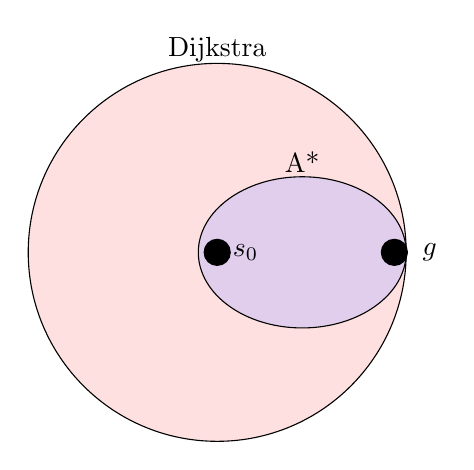
\begin{tikzpicture}[scale=0.6]
    % BrFS region

\pgfmathsetmacro{\x}{2}

\draw[fill=red!30, fill opacity=0.4] (0, 0) circle (2*\x);
\draw[fill=blue!30, fill opacity=0.4] ({0.9*\x}, 0) ellipse ({1.1*\x} and {0.8*\x});

\node[draw,circle,fill=black] (a) at (0,0) {};
\node (aa) at (0+0.6, 0) {$s_0$};

\node[draw,circle,fill=black] (b) at (2*\x-0.25,0) {};
\node (bb) at (2*\x+0.5,0) {$g$};


\node (d) at (0, 2*\x+0.3) {Dijkstra};
\node (a) at ({0.9*\x}, {0.8*\x+0.3}) {A*};

  \end{tikzpicture}
  \caption{A* (ヒューリスティック探索)とダイクストラ法 (情報なし探索)の探索範囲の比較}
\label{fig:dijkstra-astar}  
\end{figure}

ダイクストラ法は初期状態からそのノードまでのコストである$g$値が最小のノードを展開していく。これは間違った方針ではないだろうが、理想的にはゴール状態に向かっていくノードを展開していきたい。図\ref{fig:dijkstra-astar}の大きい方の円はダイクストラ法 (情報なし探索)による状態空間の探索を図示したものである。ダイクストラ法はゴールがどこにあるかということを無視して探索を進めているため、初期位置からどの方向へも均等に探索を行う。
人間の目で見れば一目で右に探索していけばよいというのは分かる。そのような人間の持っている知識を利用して探索を効率化出来ないだろうか?
\define{A*探索}{A* search}{エースターたんさく}はゴールまでの距離を見積もる\define{ヒューリスティック関数}{heuristic function}{ヒューリスティックかんすう}を用いることでゴールに向かって探索していくことを目指した手法である。

A*探索はヒューリスティック探索の代名詞である、最も広く知られている手法である \cite{fikes:71}。
A*探索は以下の$f$値が最小となるノードを優先したグラフ探索アルゴリズムである。

\begin{equation}
  f_{\text{A*}}(s) = g(s) + h(s)
\label{alg:astar-search}
\end{equation}

\begin{figure}
  \centering
  \begin{tikzpicture}[scale=0.6]
    % BrFS region

\pgfmathsetmacro{\x}{3}

\node[draw,circle,fill=black] (s0) at (0,0) {};
\node (ss) at (0, 0 - 0.6) {$u_0$};

\node[draw,circle,fill=black] (t) at (2*\x,0) {};
\node (gg) at (2*\x,0 - 0.6) {$t$};


\node[draw,circle,fill=black] (c) at (\x * 0.8, 0.5 * \x) {};
\node (cc) at (\x * 0.8, 0.5 * \x - 0.6) {$u$};


\draw[->] (s0) -- (c) node[above,pos=0.5] {$g(u)$};
\draw[->,dashed] (c) -- (g) node[above,pos=0.5] {$h(u)$};


  \end{tikzpicture}
  \caption{$f_{\text{A*}}$値の意味}
  \label{fig:fvalue}
\end{figure}


ノード$s$の$f$値は、初期状態$s_0$から$s$を通過してゴール状態$g$に辿り着くためのコストの見積もりである (図 \ref{fig:fvalue})。$g$値は初期状態からノード$s$までの既知の最短経路コストである。一方$h$値はヒューリスティック関数による$s$からゴール状態までの最短経路の見積もりである。
A*探索は非明示的グラフ探索アルゴリズム(アルゴリズム\ref{alg:implicit-graph-search})の一つであり、$f$値が最小ノードから優先して探索を行う \ref{alg:astar-search}。

% $g(n)$のみでノードを選択するダイクストラ法(\ref{sec:dijkstra}章)と比較すると、A*探索はゴール状態までのコストの見積もりを考慮して次に展開するノードを決めている。

% 図\ref{fig:grid-astar-mdheuristic}は\define{マンハッタン距離ヒューリスティック}{Manhattan distance heuristic}{マンハッタンきょりヒューリスティック}によるA*探索である。
% 青いノードは展開済みノード、緑のノードはオープンリストに入れられた未展開ノードである。幅優先探索による図\ref{fig:grid-dijkstra}と比較すると、展開済み・未展開ノードの数が少なく済んでいることがわかるだろう。


\dtheorem{
  グラフに経路コストが0以下のサイクルが存在しない場合、A*は完全である。  
}
\dproof{
  グラフが有限である場合は、やがてすべてのノードを生成・展開し解を発見するので、完全である。
  グラフが無限である場合もやがて解を発見できる。最適解のコストを$c^*$とすると、A*が展開するノードは$f(s) \leq c^*$のノードのみである。本書ではグラフは局所有限であると仮定している (すべてのノードの分枝数は有限である)ので、$f(s) \leq c^*$を満たすノードは有限個である。A*探索はやがてこれらのノードをすべて生成・展開し解を発見するので、完全である。
}
なお、解が存在しない場合、グラフが無限である場合にA*は停止しないので停止性を満たさない。


A*に用いるヒューリスティック関数は正確であるほど良いが、それに加えて許容的、無矛盾であるという性質も有用である。

\dtheorem{
ヒューリスティックが許容的である時、A*は最適解を返す。
}
\dproof{

%全てのノードnは展開時にg(n)がnに辿り着くための最短経路コストの値である。%これは無矛盾性か
許容的なヒューリスティック$h(n)$は$n$からゴールへの経路の下界である。よって、ゴール状態の$h$値は$0$である。つまりゴール状態の$f$値は$g$値と同じである。この解の$g(n')$値を$f*$と置く(解のコストに相当)。
A*のノードの展開順に従うと、$f*$のノードを展開する前に全ての$f<f*$のノードが展開される。
これらのノードがいずれもゴール状態でなければ、$g(n) \leq f(n)$より、$g(n)<f*$となるゴール状態がない。すなわち、$f*$が最適解のコストとなり、$n'$がその時のゴール状態である。

}

A*探索はノードの\define{再展開}{reexpansion}{さいてんかい}が生じる可能性がある。
アルゴリズム\ref{alg:implicit-graph-search}にあるように、すでに訪れた状態に再び訪れたとき、前に訪れたときよりも小さな$g$値で訪れた場合、ノードを再展開する。このとき、その状態から先の部分木もより小さな$g$値で訪れることになるので、部分木をすべて更新しなければならない。そのため、ノードの再展開によってかなり性能が落ちてしまうことがある。
無矛盾なヒューリスティックの魅力はA*で再展開が生じないことにある。

\dtheorem{
無矛盾なヒューリスティックを用いたA*探索はノードの再展開が生じない。
}

無矛盾なヒューリスティックである場合、A*探索は全てのノード$n \in S$に最初に最短経路コストで訪れることが証明できる。そのため再展開が生じない。

効率的なA*探索のためには良いヒューリスティック関数をデザインしたい。
許容的で無矛盾なヒューリスティックであると解析的に良い性質を満たしていると言える。
一方、経験的に速いと知られているヒューリスティック関数の中にはこれらの性質を満たしていないものも多い。


A*に用いるヒューリスティック関数は正確であるほどより探索範囲を狭めることができる。

\ddef{ヒューリスティックの情報} {
  ヒューリスティック$h_1$とヒューリスティック$h_2$が両方許容的であり、かつすべてのゴールでない$s \in S$に対して
  \begin{equation}
    h_2(s) > h_1(s)
  \end{equation}
  であるとき、$h_2$は$h_1$よりも\define{情報がある}{more informed}{ヒューリスティックのじょうほう}と呼ぶ。
}

より情報があるヒューリスティックを使う方がA*は効率的である。

\dtheorem{
  (ノード展開の必要条件): A*探索で展開されるノードの$f$値はすべて最適解のコスト以下である ($f(s) \leq c^*$)。
}

\dtheorem{
  (ノード展開の十分条件): $f$値が最適解のコスト未満であるノードは必ずすべてA*探索で展開される ($f(s) < c^*$)。
}

A*探索は$f$値が一番小さいノードから展開していくので、これらの定理が満たされる。

\dtheorem{
  $h_2$が$h_1$よりも情報がある場合、$h_2$を使ったA*探索によって展開されるノードはすべて$h_1$を使ったA*探索でも展開される。
}
\dproof{
  $h_2$によるA*で展開されるノードの集合はすべて$c^* \geq g(s) + h_2(s)$である。
  ゴールを除き$g(s) + h_2(s) > g(s) + h_1(s)$である。
  よって、$c^* > g(s) + h_1(s)$なのでこれらのノードはすべて$h_1$を使ったA*探索でも展開される。
} 

よって、A*に使うヒューリスティックは情報があるほど良い。


一方のヒューリスティック関数が他方より情報がある場合はより情報のある方を使えばよい。
しかし、ある場所では$h_1$よりも$h_2$の方が正確であり、他のある場所では$h_2$よりも$h_1$の方が正確である、となる場合がある。この場合どちらのヒューリスティックを使えば良いだろうか?実は両方を使うことによってより良い正確なヒューリスティックを得ることができる。

\dtheorem{
  %\begin{itemize}
    ヒューリスティック$h_1,..., h_m$が許容的であるとき、$h(s) = \max(h_1(s),..., h_m(s))$は許容的である。
    ヒューリスティック$h_1,..., h_m$が許容的で無矛盾であるとき、$h(s) = \max(h_1(s),..., h_m(s))$は許容的で無矛盾である。
  %\end{itemize}
}

このように複数のヒューリスティックを組み合わせることでより良いヒューリスティックを得ることができる。
このアイディアはさまざまなヒューリスティック関数の自動生成に応用されている。


\section{ヒューリスティック関数の例}
\label{sec:heuristic-example}

\ref{sec:heuristic-function}章にあるように、なるべく正確であり、許容的、無矛盾なヒューリスティックが望ましい。
一般に、許容的なヒューリスティックを得る方法としては、元問題の{\bf 緩和問題}を解き、その最適解コストをヒューリスティック値とすることである。ある問題の緩和問題とは、解集合に元の問題の解を含む問題を指す。要するに元の問題より簡単な問題である\footnote{解が多いほど簡単であるとは一概には言えないが}。
グラフ探索アルゴリズムにおいて緩和問題を作る方法は様々あるが、一つはグラフのエッジを増やすことで緩和が出来る。グラフのエッジを増やすには、問題の可能なアクションを増やすなどの方法がある。

\subsection{グリッド経路探索:マンハッタン距離}

4方向グリッド経路探索問題の元問題は障害物のあるグリッドに移動することは出来ない。グリッド経路探索で有効なヒューリスティックの一つはマンハッタン距離ヒューリスティックである。これは現在位置とゴール位置のマンハッタン距離を$h$値とする。マンハッタン距離は障害物を無視した最短経路の距離であるので、元の問題グラフに対してグラフのエッジを増やした緩和問題での解のコストに対応する。
このように、問題の性質を理解していれば許容的なヒューリスティック関数を設計することが出来る。


\subsection{スライディングタイル:マンハッタン距離}
スライディングタイルにおけるマンハッタン距離ヒューリスティックは各タイルの現在の位置とゴール状態の位置のマンハッタン距離の総和を$h$値とする。
スライディングタイル問題において一度に動かせるタイルは1つであり、その距離は1つである。
そのため、マンハッタン距離ヒューリスティックは許容的なヒューリスティックである。

\subsection{スライディングタイル:パターンデータベース}

\define{パターンデータベースヒューリスティック}{Pattern database heuristic}{パターンデータベースヒューリスティック}は部分問題を解き、その解コストをヒューリスティック値とするアルゴリズムである\cite{edelkamp2001planning}。
探索を始める前に部分問題を解き、部分問題のすべての状態からゴール状態への最適解のコストをテーブルに保存する。
図\ref{fig:pattern-database}はスライディングタイルにおけるパターンデータベースの例である。
図の例は「1, 2, 3, 4のタイルを正しい位置に動かす」という部分問題を解いている。
この部分問題では5, 6, 7, 8のタイルの位置はどこでもよい。1, 2, 3, 4さえゴール位置にあればよい。
ゴール条件以外は元の問題と同様である。
この部分問題は元の問題の緩和問題になっているので許容的なヒューリスティックが得られる。

図の例では1, 2, 3, 4のタイルに絞った部分問題だったが、他のタイルの組み合わせでも良い。
例えば1, 2, 3, 4のタイルによる部分問題と5, 6, 7, 8のタイルによる部分問題からは異なるヒューリスティック値を得ることができる。
これらのヒューリスティック値の最大値を取ることでより正確なヒューリスティックにすることができる。
このように複数のパターンデータベースを使うヒューリスティックを\define{複数パターンデータベース}{multiple pattern databse}{ふくすうパターンデータベース}と呼ぶ。複数パターンデータベースは一つの大きなパターンデータベースを使うよりも正確さに欠けるが、計算時間・空間の面で大きなアドバンテージがある。

1, 2, 3, 4のタイルによる部分問題と5, 6, 7, 8のタイルによる部分問題は一見完全に分割された部分問題なので、これらのヒューリスティック値の和を取ってもよさそうだが、そうすると許容的なヒューリスティックにはならない。なぜなら例えばタイル5を動かすアクションによるコストは両方の部分問題のコストに数えられているからである。
そこで部分問題のコストを「1, 2, 3, 4 (あるいは5, 6, 7, 8)のタイルを動かすときのみコストがかかり、他のタイルはコスト0で動かせる」とすると、コストを重複して数えることはなくなる。そうするとこれらの部分問題のコストの和は許容的なヒューリスティックになる。
このように複数のパターンデータベースで重複してコストが数えられないようにしたものを\define{素集合パターンデータベース}{disjoint pattern databse}{そしゅうごうパターンデータベース}と呼ぶ \cite{korf2002}。 % TODO: good term?

マンハッタン距離ヒューリスティックは、各タイルごとの部分問題8つに分けた場合の素集合パターンデータベースである。

\begin{figure}
  \centering
  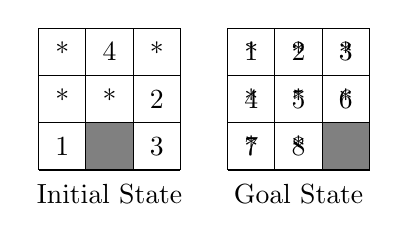
\begin{tikzpicture}[scale=0.6]
    
%%% Initial state

\draw (0, 0) grid (3, 3);


\node at (0 + 0.5, 0 + 0.5) {1};
\draw[fill=gray] (1,0) rectangle (2, 1);
\node at (2 + 0.5, 0 + 0.5) {3};

\node at (0 + 0.5, 1 + 0.5) {*};
\node at (1 + 0.5, 1 + 0.5) {*};
\node at (2 + 0.5, 1 + 0.5) {2};

\node at (0 + 0.5, 2 + 0.5) {*};
\node at (1 + 0.5, 2 + 0.5) {4};
\node at (2 + 0.5, 2 + 0.5) {*};

\node at (1.5, -0.5) {Initial State};

%%% Goal state
\pgfmathsetmacro{\base}{4}

\draw (\base+0, 0) grid (\base+3, 3);

\foreach \x in {0,...,2}
{
  \foreach \y in {0,...,2}
  {
        \pgfmathsetmacro{\val}{int(\x+3*\y+1)}
        \ifthenelse{\x=2 \AND \y=2}{;}{
          \ifthenelse{\val>4}{
            \node at (\base+\x + 0.5, 2 - \y + 0.5) {*};
          }{
            \node at (\base+\x + 0.5, 2 - \y + 0.5) {\val};
          }
        }
  }
}
\draw[fill=gray] (\base+2,0) rectangle (\base+3, 1);

\node at (\base+1.5, -0.5) {Goal State};

  \end{tikzpicture}
\caption{パターンデータベースの初期状態 (左)とゴール条件 (右)の例。1, 2, 3, 4のタイルだけゴール位置にあればよく、他のタイルの位置は関係ない。}
\label{fig:pattern-database}
\end{figure}


\subsection{巡回セールスパーソン問題:最小全域木}
TSPの解の下界としては\define{最小全域木}{minimum spanning tree}{さいしょうぜんいきき}のコストがよく用いられる (図\ref{fig:tsp-mst})。
グラフの\define{全域木}{spanning tree}{ぜんいきき}は全てのノードを含むループを含まない部分グラフである。
最小全域木は全域木のうち最もエッジコストの総和が小さいものである。
未訪問の都市によるグラフの最小全域木はTSPの下界となることが知られている。
ヒューリスティック探索ではまだ訪問していない都市をカバーする最小全域木のコストをヒューリスティック関数に用いる。
最小全域木は素早く計算ができるので探索には使いやすい。

\begin{figure}[tbh]
  \centering
  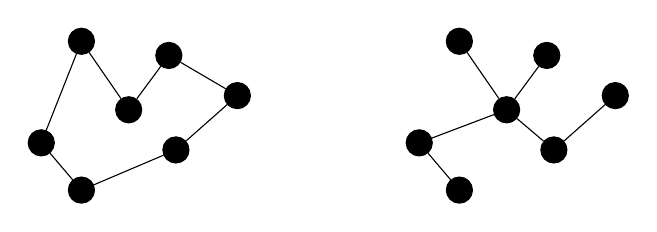
\begin{tikzpicture}[scale=0.6]
    \foreach \x in {0, 8}
  {
    \pgfmathsetmacro{\noise}{0.15}           
\node[draw,circle,fill=black] (1\x) at (\x+0, 0) {};
\node[draw,circle,fill=black] (2\x) at (\x+2, 1-\noise) {};
\node[draw,circle,fill=black] (3\x) at (\x+3+2*\noise, 2) {};
\node[draw,circle,fill=black] (4\x) at (\x+2-\noise, 3-\noise) {};
\node[draw,circle,fill=black] (5\x) at (\x+1, 2-2*\noise) {};
\node[draw,circle,fill=black] (6\x) at (\x+0, 3+\noise) {};
\node[draw,circle,fill=black] (7\x) at (\x-1+\noise, 1) {};
}

% TSP Solution
\foreach \a in {1,...,6}
  {
    \pgfmathsetmacro{\n}{int(\a+1)}
    \draw[-] (\a0) -- (\n0);
  }

\draw[-] (70) -- (10);

% Minimum spanning tree

\draw[-] (18) -- (78);
\draw[-] (28) -- (58);
\draw[-] (38) -- (28);
\draw[-] (48) -- (58);
\draw[-] (58) -- (68);
\draw[-] (78) -- (58);

  \end{tikzpicture}
\caption{巡回セールスパーソンにおけるTSP解 (左)と最小全域木 (右)}
\label{fig:tsp-mst}
\end{figure}


\section{非最適解の探索}
\label{sec:inadmissible}

許容的なヒューリスティックを用いたA*探索は最適解が得られるが、必ずしも最適解がほしいわけではない場合もある。解のクオリティよりもとにかく解が何か欲しい、という場合もある。
最適解ではない解を\define{非最適解}{suboptimal solution}{ひさいてきかい}と呼び、最適解に限らず解を発見するアルゴリズムを\define{非最適探索}{suboptimal search}{ひさいてきたんさく}と呼ぶ。% あるいは\define{局所探索}{local search}と呼ぶ。 % 局所探索はまた違う文脈か

\subsection{重み付きA*探索 (Weighted A*)}
\label{sec:weighted-astar-search}

\define{重み付きA*探索}{weighted A*}{おもみつきエースターたんさく} (wA*)は解のクオリティが落ちる代わりにより素早く解にたどり着くための手法である \cite{wilt2010comparison}。
wA*は重み付き$f$値、$f_w$が最小のノードを優先して探索する。

\begin{equation}
	f_w(n) = g(n) + w h(n)
\end{equation}

\dtheorem{
許容的なヒューリスティックを用いた重み付きA*探索によって発見される解は最適解のコスト$f^*$の$w$倍以下である。
}


wA*の利点はA*よりもはるかに高速であることである。
多くの場合、$w$の大きさに対して指数的な高速化が期待できる。これは深さ$d$のノードの個数は$d$に対して指数的(分枝度を$b$とすると$b^d$個)であることに対応する。

wA*などの非最適探索を使う場合はいずれにせよ最適解が得られないので、許容的でないヒューリスティックと組み合わせて使われることが多い。許容的でないヒューリスティックは許容的なヒューリスティックよりも高速であることが多い。% TODO lama?

wA*の解は最適解のコストの上界になるので、A*探索の枝刈りに用いることが出来る。
A*探索を実行する前にwA*を走らせ、解の上界$c^*$を得、A*探索実行時にノード$n$に対して$f$値が$f(n) \geq c^*$である場合、そのノードを枝刈りすることができる。このテクニックは多重配列アライメントなどに使われる\cite{ikeda1999enhanced}。

図\ref{fig:grid-astar}、\ref{fig:grid-wastar}はグリッド経路探索問題でのA*とwA* ($w=5$)の比較である。
緑のグリッドが初期位置、赤のグリッドがゴール、黒のグリッドは進行不可能の壁である。
青のグリッドが探索終了時点に各アルゴリズムによって展開されたノード、薄緑のグリッドが各アルゴリズムに生成され、まだ展開されていないノード (オープンリストにあるノード)である。

wA*の展開・生成ノード数がA*よりも少ない。
ただしwA*で発見された解はA*で発見された解よりも遠回りなことがわかる。
A*探索は最適解を発見するが、wA*では最初に発見した解が最適とは限らない。

\begin{figure}
  \centering
  \subfloat[A*] {
    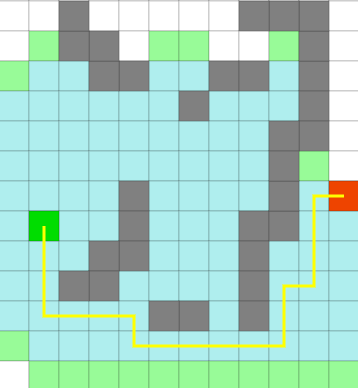
\includegraphics[width=0.3\linewidth]{./figures/grid-astar.png}
    \label{fig:grid-astar}
  } \hspace{4pt}
  \subfloat[wA*] {
    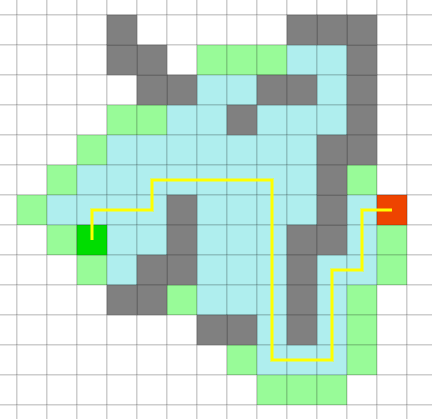
\includegraphics[width=0.3\linewidth]{./figures/grid-wastar-5.png}
    \label{fig:grid-wastar}
  } \hspace{4pt}
  \subfloat[GBFS] {
    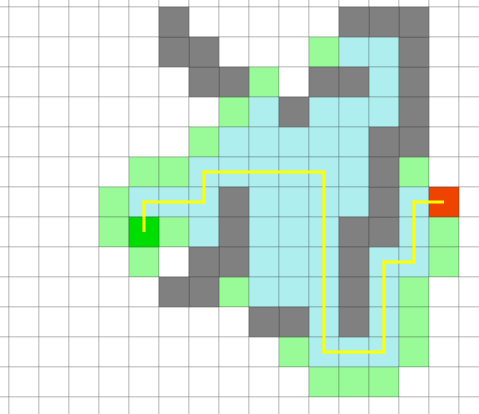
\includegraphics[width=0.3\linewidth]{./figures/grid-gbfs.png}
    \label{fig:grid-gbfs}
  }
  \caption{グリッド経路探索問題におけるA*、wA*、GBFSの比較}
  \label{fig:grid-comparison}
\end{figure}

\subsection{貪欲最良優先探索 (Greedy Best-First Search)}
\label{sec:greedy-best-first-search}

wA*の例で見たように、$g$値に対して$h$値に重きを置くことによって解のクオリティを犠牲により高速に解を得ることができる。
問題によっては解のクオリティはあまり重要でなかったり、そもそもクオリティという概念がないことがある。
このようにとにかく解があればよいという場合は\define{貪欲最良優先探索}{Greedy Best-First Search}{どんよくさいりょうゆうせんたんさく}が使われることが多い \cite{wilt2010comparison}。

\begin{equation}
  f_{\text{gbfs}}(s) = h(s)
\end{equation}

貪欲最良優先探索は$g$値を無視し、$h$値のみで展開順を決定する。つまりwA*の$w$を無限大にしたものである。

貪欲最良優先探索は解のクオリティに保証がない。
しかし多くの問題で高速に解を発見できるとても強力な手法である。
図\ref{fig:grid-gbfs}は貪欲最良優先探索である。wA*よりもさらに生成ノード数が少ないことが分かるだろう。

\subsection{山登り法 (Hill Climbing)}
\label{sec:hill-climbing}

A*探索はクローズドリストに探索済みのノードを記憶しておくことでグラフ全体を見渡して探索を進める。しかし探索済みのノードをメモリにおいておくことは時間がかかるし、メモリも消費する。\define{局所探索}{local search}{きょくしょたんさく}は現在見つかった最良のノードのみを記憶しておくことで効率的に(最適とは限らない)解を発見する方法である。

\define{山登り法}{hill climbing}{やまのぼりほう}は局所探索アルゴリズムであり、特に組み合わせ最適化問題のためのアルゴリズムとして使われる。
山登り法のアルゴリズムは非常に単純である。子ノードのうち最も$h$値が小さいノードを選ぶことを繰り返す。

\begin{algorithm}
\caption{山登り法 (Hill Climbing)}
	\Input{非明示的状態空間グラフ $(s, Goal, Expand, w)$, 評価関数 $h$}
	\Output{$s$からゴール状態$t \in T$への経路、経路が存在しなければ$\emptyset$}
	\While {{\bf not} $Goal(s)$} {
	  $u \leftarrow \arg \min_{s' \in Expand(s)} h(s')$\;
          $parent{u} \leftarrow s$\;
          $s \leftarrow u$\;
	}
	\Return $Path(s)$
\label{alg:hill-climbing}
\end{algorithm}

この手法は組合せ最適化・連続最適化のためによく使われる。
グラフ探索アルゴリズムでこのまま使おうとすると評価関数の極小ではまってしまったり、デッドエンドに落ちてしまう可能性がある。


\subsection{強制山登り法 (Enforced Hill Climbing)}

ヒューリスティック探索でよく使われる局所探索は\define{強制山登り法}{enforced hill-climbing}{きょうせいやまのぼりほう} (EHC)である \cite{hoffmann2005ignoring}。
EHCは幅優先探索を繰り返し、現在のノードよりも$h$値が小さいノードを発見する。発見できればそのノードから再び幅優先を行い、ゴールを発見するまで続ける。もし$h$値が小さいノードが見つからなければ極小に陥ってしまったということであるので、探索を打ち切り、失敗 (Fail)を返す。

\begin{algorithm}
\caption{強制山登り法 (Enforced Hill Climbing)}
	\Input{非明示的状態空間グラフ $(s, Goal, Expand, w)$, 評価関数 $h$}
	\Output{$s$からゴール状態$t \in T$への経路、経路が存在しなければ$\emptyset$}
	\While {{\bf not} $Goal(s)$} {
	  $T \leftarrow \{v \in Expand(s)\}$\;
	  $T' \leftarrow \{v \in T | h(v) < h(s) \}$\;
          \While {$T' = \emptyset$} {
            $T \leftarrow \{v \in Expand(u) | u \in T\}$\;
 	    $T' \leftarrow \{v \in T | h(v) < h(s) \}$\;
          }
	  $u \leftarrow \arg \min_{s' \in Expand(s)} h(s')$\;
          $parent(u) \leftarrow s$\;
          $s \leftarrow u$\;
	}
	\Return $Path(s)$
\label{alg:enforced-hill-climbing}
\end{algorithm}


ほとんどの局所探索アルゴリズムは完全性を満たさない。
なので解が発見できなければ(失敗を返す場合)続けてA*探索などを走らせないと解が発見できない場合がある。
山登り法などの局所探索の利点はなんといってもアルゴリズムはシンプルであり、実装が簡単であることである。
また、オープンリストなどのデータ構造を保持する必要がないので消費メモリ量が非常に少ない。

山登り法が記憶しなければならないノードは現在のノードとその子ノードらだけである。
毎回次のノードを選択したら、そのノード以外のノードは捨ててしまう。
貪欲最良優先探索(\ref{sec:greedy-best-first-search}節)も同様に$h$値のみしか見ていないが、すべての生成済みノードをオープンリストに保存して評価値を確認していることと比較すると、山登り法がいかにアグレッシブな手法であるかがうかがえるだろう。

\section{上手く行かない場合}

ヒューリスティック探索が思ったより遅い場合考えるべきことはいくつかある。

まず考えるべきは、そもそもヒューリスティック探索によって解くべき問題なのかという点である。
制約プログラミングや他の組合せ最適化手法なら効率的な問題かもしれない。
似たような問題が他の手法によって解かれていないかを調べてみると良い。

ヒューリスティック探索が良さそうだと思ったら、試しにwA*にしてみて、weightを大きく取ってみよう。
おおまかに言うとwA*の実行速度はwの大きさに対して指数的に速くなる。$w=1$だと全く解けそうにない問題でも$w=2$にすると一瞬で解けることがある。
もし$w$を10くらいにしてもすぐに解が発見できなければ、おそらくその問題で最適解を発見するのは非常に難しい。このような問題に対しては最適解を見つけることは諦め、非最適解探索 (節 \ref{sec:inadmissible})を使ったほうが良いだろう。
wA*でも解が見つけられない場合はそもそも解がない問題かもしれない。解がない場合は制約プログラミングのソルバーを使うと素早く検出できることが多い。

wA*で非最適解を見つけられる場合なら、工夫すればA*で最適解を見つけることができるかもしれない。
その場合まず、おおまかな探索空間の大きさを見積もり、そして1秒間に何ノードが展開されているかを確認すると良い。
ヒューリスティック探索の実行時間はおおまかには(展開するノード数)と(1ノードの展開にかかる時間)の積である。

%例えばA*探索はC++でスライディングタイル問題だと秒間XXXノードが展開できる。
もし秒間に展開されているノードの数が少ない場合、プロファイラを使ってどのオペレーションに時間がかかっているかを確認するべきだろう。多くの場合実行時間の大半をオープンリスト、クローズドリスト、ノードの展開関数(現在の状態とアクションから状態を計算する関数)のいずれかが占めている、ということがわかるだろう。

オープンリスト、クローズドリストの処理に時間がかかっている場合はデータ構造の改良によって問題が解決するかもしれない。効率的なデータ構造の設計については\ref{ch:search-performance}章を参照されたい。
特に探索が進みデータ構造が大きくなるほどアクセスするためにかかる時間がどんどん増えていく場合はデータ構造の工夫によって解決できる可能性がある。
あとはプロセスのメモリ消費量を確認してみよう。A*はメモリ消費も激しい。
実行時間が遅いのは、メモリを使いすぎていてメモリスワップが起きているからかもしれない。
より大きなメモリを使うか、IDA*などのメモリの消費量の少ない手法を試してみると良いかもしれない。

ノードの展開関数に時間がかかる場合はその実装を工夫するか、ノードの展開回数を最小限に抑えるしかない。
ノードの展開回数を減らす方法はなかなか難しいが、例えばヒューリスティック関数の改良によって可能である。
ほんの少しのヒューリスティック関数の改善によって探索の効率は劇的に上がりうる。
% 例えばスライディングタイル問題ではTODO。

これらの方法でもまだ解けない場合、扱っている問題は純粋なA*で解くには結構難しい問題かもしれない。
1968年にA*が初めて提案されてから、様々な発展手法が考案されてきた。
本書の後半で紹介する最新の手法を試してみれば解けるかもしれない。


\section{Python実装}

A*探索の実装は非常にシンプルである。グラフ探索のコードに渡すプライオリティ関数を$f = g + h$にすればよいだけである。

\inputpython{python/astar_search.py}{1}{5}

重み付きA*や貪欲最良優先探索もほぼ同様である。

\inputpython{python/wastar_search.py}{1}{5}
\inputpython{python/greedy_best_first_search.py}{1}{5}

ヒューリスティック関数の実装は問題によっては難しい場合もある。
ここではグリッド経路探索のためのマンハッタン距離ヒューリスティック関数を紹介する。

\inputpython{python/grid_pathfinding.py}{66}{68}

この関数を\code{GridPathfinding}クラスに追加すればよい。
スライディングタイル問題のためのマンハッタン距離ヒューリスティック関数は以下のようになる。

\inputpython{python/sliding_tile.py}{78}{93}

各問題に対してそれぞれのヒューリスティック関数を実装することは面倒に感じられるかもしれない。
ある特定の問題に特化して高速化させたい場合は、ヒューリスティック関数はその問題の前提知識を利用した関数であるので、それぞれの問題毎に適切なものを実装する必要があるだろう。
一方で汎用的に様々な問題に対して使えるヒューリスティック関数もあるので、\ref{ch:classical-planning}章で紹介する。


\section{まとめ}

状態空間問題に対して何らかの前提知識がある場合、その知識を利用して探索を効率化させる方法の一つとしてヒューリスティック探索がある。
ヒューリスティック探索は状態の「有望さ」を推定できる場合、それをヒューリスティック関数として表すことが出来る。

ヒューリスティック探索で基本となる手法はA*探索である。
A*は各ノードの有望さをそのノードに到達するまでのコストとそのノードからゴールに到達するまでのコストの推定値の和として推定し、最も有望なノードから優先して探索する手法である。

ヒューリスティック関数のうち重要な性質は2つある。
許容的なヒューリスティック関数はゴールまでのコスト未満の推定をしないヒューリスティックであり、これを用いたA*は最適解が見つけられることが保証されている。
無矛盾なヒューリスティックを用いたA*探索はノードの再展開が生じない。

A*で解を見つけるのに時間がかかりすぎる場合は、最適解を見つけることを諦めてwA*や局所探索を用いることができる。

\section{練習問題}

\begin{enumerate}
  \item グリッド経路探索問題においてマンハッタン距離ヒューリスティックを実装し、A*探索を実装せよ。幅優先探索と比較して展開するノードの数は変わったか。

  \item グリッド経路探索問題において、グリッドが斜めを含めた隣り合う8マスに動ける場合を考える。このとき、現在位置とゴール位置とのマンハッタン距離は許容的である。では、現在位置とゴール位置とのユークリッド距離 (直線距離) は許容的なヒューリスティックになるか?
  
  \item 斜め移動ありのグリッド経路探索問題においてマンハッタン距離よりも推定値が正確でありかつ許容的なヒューリスティック関数はあるだろうか?
  (ヒント:ある。)
  
  \item 上述のヒューリスティック関数を用いたA*探索で斜め移動ありのグリッド経路探索問題を解いてみよう。マンハッタン距離を用いた場合と比較して展開するノードの数は変わったか。
  
  \item ヒューリスティック$h$が許容的であるとする。このとき、$h'(s) = h(s) + c$は許容的であるか?$c$が何を満たせば許容的であるか?($c$は定数とする)
  \item ヒューリスティック$h$が無矛盾であるとする。このとき、$h'(s) = h(s) + c$は無矛盾であるか?$c$が何を満たせば無矛盾であるか?($c$は定数とする)
  
  \item 「許容的なヒューリスティックを用いた重み付きA*探索によって発見される解は最適解のコスト$f^*$の$w$倍以下である」ことを証明せよ。
  (ヒント: 「ヒューリスティックが許容的である時、A*は最適解を返す」定理の証明が参考になる。)
  
  \item 山登り法が解を見つけることが出来ないような状態空間問題の例を一つ考えてみよう。
\end{enumerate}


\section{関連文献}

\define{最良優先探索}{best-first search}{さいりょうゆうせんたんさく}は2種類の定義があることに注意したい。
本書では最良優先探索をA*を含む、何らかの有望さの指標に従ってグラフを探索するアルゴリズムを指す。
一方、ゴールに最も近いと考えられるノードを常に最優先して展開するアルゴリズムを特に最良優先探索と呼ぶことも多い。本書ではこの方法は貪欲最良優先探索と呼んでいる。

制限時間内でできるだけ良いクオリティの解が欲しい場合はAnytime Reparing A* \cite{likhachev2004ara}が使える。Anytime Reparing A*は問題に対して重み付きA*を繰り返し$w$値をだんだんと小さくしていくことでだんだんと解のクオリティを向上させる。一般にいつ停止しても現時点で見つかった中で一番良い (最適とは限らない)解を返し、時間をかけるほど解のクオリティを改善していくアルゴリズムをanytimeアルゴリズムと呼ぶ。Anytimeアルゴリズムとしては他にもモンテカルロ木探索などがある \cite{browne2012survey}。

山登り法は評価値が最も良い状態を決定論的に選ぶので解・最適解を発見する保証はない。
一方、すべての次状態を均等な確率でランダムに選ぶランダムウォークはいずれ解を発見するが、時間がかかりすぎる。
\define{焼きなまし法}{simulated annealing}はこの二つの手法の中間をとったような手法であり、最初は評価値を無視して均等なランダムウォークからはじめ、探索が進行していくにつれて評価値に応じて次状態を選択するようにするという手法である \cite{vcerny1985thermodynamical,van1987simulated}。焼きなまし法は最適化問題で非常に重要なアルゴリズムである \cite{kirkpatrick1983optimization}。

\define{遺伝的アルゴリズム}{genetic algorithm}もさまざまな最適化問題に適用できる重要なアルゴリズムである \cite{goldberg1989}。
グラフ探索問題で使われることは少ないが、グラフ探索問題ではなかなか解けない難しい問題が遺伝的アルゴリズムによって簡単に解けることがある。例えばN-Queen問題はチェスの盤面上にクイーンを互いに移動可能範囲がぶつからないように配置する問題であるが、これはグラフ探索の手法だとなかなか解くのが難しいが遺伝的アルゴリズムだと非常に効率的に解けることが知られている。
